\section{Introduction}
\label{sec:intro}	
\IEEEPARstart{A}{nomaly} detection has profound impacts on preventing malicious activities in various applications, such as detecting online review spams~\cite{nabeel2021cadue}, financial frauds~\cite{SemiGNN,liang2019uncovering}, fake users~\cite{fawcett1996combining}, and misinformation~\cite{cui2020deterrent, silva2021propagation2vec}. 
The most promising development is to utilizing graph structures via machine learning models for distinguishing the anomalies from normal nodes, as graphs can be used for modeling the structural dependencies underlying the data~\cite{kumar2018rev2,liu2020alleviating,dou2020enhancing}. 

%For example, studies have shown that in online review platforms, the structure of the user-item graph plays a critical role in identifying fraudulent users~\cite{kumar2018rev2,liu2020alleviating,dou2020enhancing}. 


%A significant line of works has been focused on discovering and incorporating the structural and attributive patterns of anomalies into learning the classification-based models~\cite{akoglu2015graph, rayana2015collective, kumar2018rev2}.
Recently, the advances of graph neural networks (GNNs)~\cite{kipf2016semi,velivckovic2017graph,Graphsage} have inspired and empowered various attempts to adopt GNNs for detecting anomalies~\cite{liu2020alleviating,dou2020enhancing,shi2022h2,SemiGNN, huang2022auc}. 
%The recent advances of graph neural networks (GNNs), such as GCN~\cite{kipf2016semi}, GAT~\cite{velivckovic2017graph}, GraphSAGE~\cite{hamilton2017inductive}, and GIN~\cite{xu2018powerful}, have promoted the graph-based anomaly detection models. 
%For example, GraphConsis~\cite{liu2020alleviating} and CARE-GNN~\cite{dou2020enhancing} are proposed for review fraud detection, GeniePath~\cite{liu2019geniepath} and SemiGNN~\cite{SemiGNN} are for financial fraud detection, and ASA~\cite{AsAWWW} is for mobile fraud detection. 
The main idea of GNN-based anomaly detection is to leverage the power of GNNs to learn expressive node representations with the goal of distinguishing abnormal nodes from normal ones in the embedding space. Most of the GNN models are based on the inductive bias that two neighboring nodes tend to have the same labels. However, suspicious links between abnormal and normal nodes violate the above assumption, making GNNs produce confusing node embeddings.   
%However, such anomalies violate the class-homophily assumption in the graph --- two neighboring nodes tend to have similar features and same labels --- via suspicious links, i.e., the links between abnormal and normal nodes, which hinders the representation model to learn the accurate node embeddings, and also the classier to construct a hyperplane to differentiate abnormal and normal nodes effectively. 

%which agrees with the claims of~\cite{wei2021crest, yang2020rethinking}, the class-imbalance problem。
%formulate anomaly detection as the node binary classification problem, and then leverage the graph structures to propagate the node embeddings along the links, finally predict the node labels based on their embeddings. 
%Most of them revise the message passing process between neighbors in the general GNNs, because the homophily assumption between neighbors might be violated between the normal and abnormal nodes. For example, a wrong paper of a researchers may still have the same-coauthor relationships with the right papers, and fraudsters may comment the same items with the benign users. The links that connect nodes with different labels are named as suspicious links, which are regarded as the key challenges to be addressed by existing GNN models.  


% To further understand the behavior of anomalies, we take the author ``Jos Rodriguez" from the academic dataset used in KDD CUP 2013\footnote{\url{https://www.kaggle.com/c/kdd-cup-2013-author-paper-identification-challenge/data}} as a case study by building a graph with papers assigned to him as nodes, and connect two papers with an edge if they share the same coauthors or venues. 

% \begin{figure}[t]
% 	\centering
% 	%\hspace{-0.2in}
% 	%\subfigure[AMiner]{\label{subfig:paper_network}
% 	%	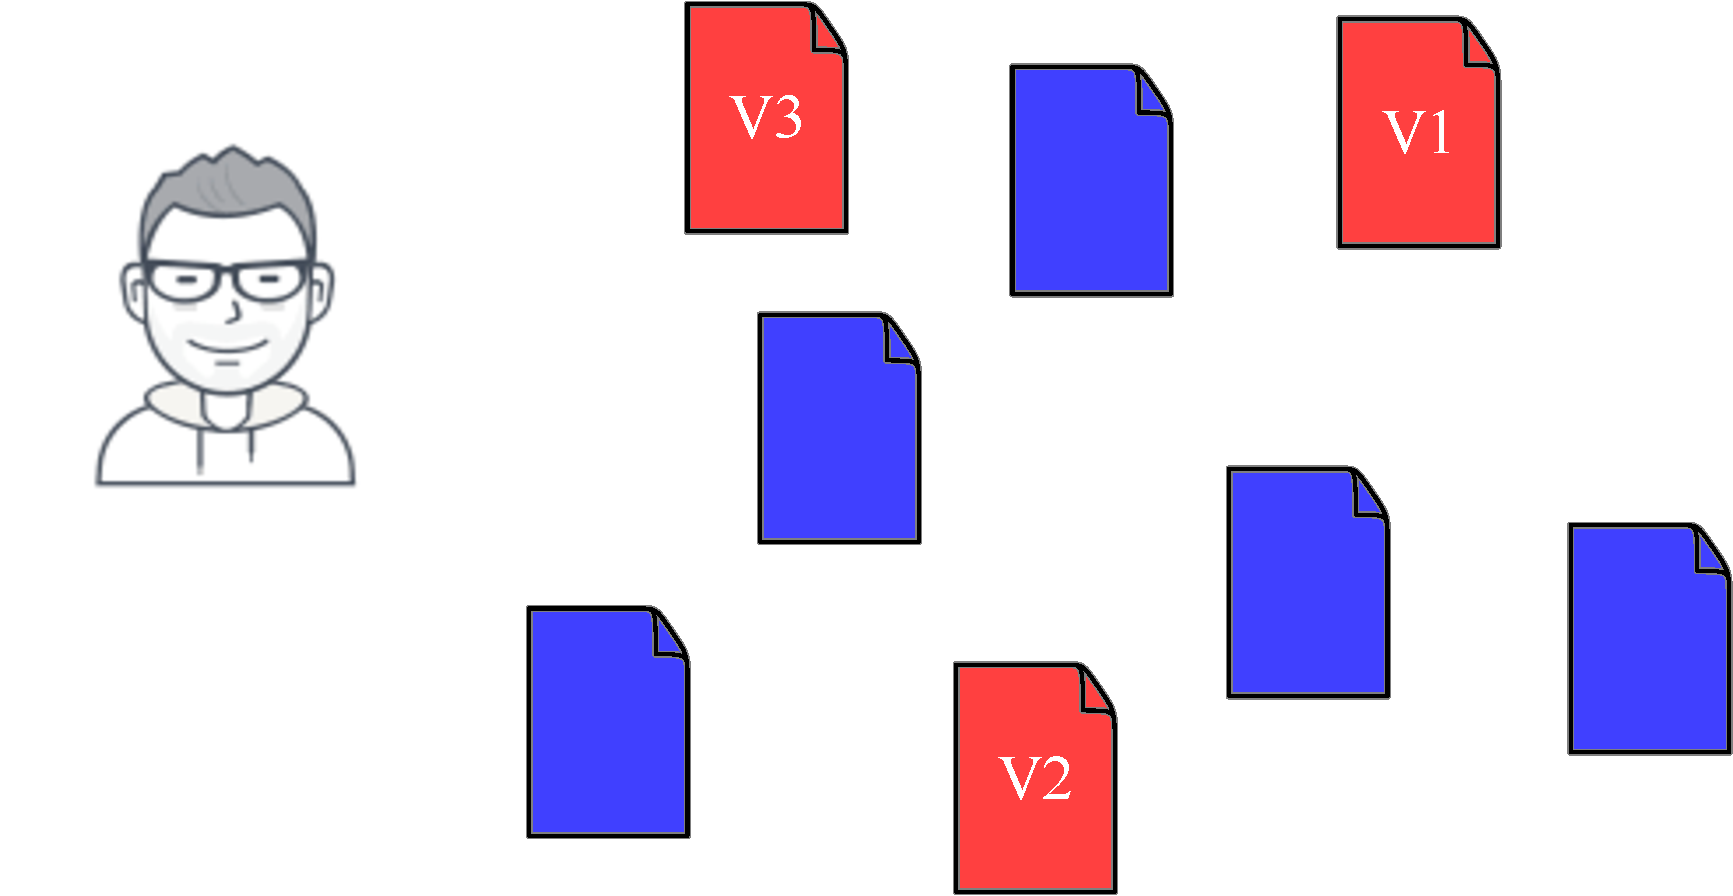
\includegraphics[width=0.33\textwidth]{figures/motivation}
% 	%}
% 	\subfigure[t-SNE]{\label{subfig:t-sne}
% 		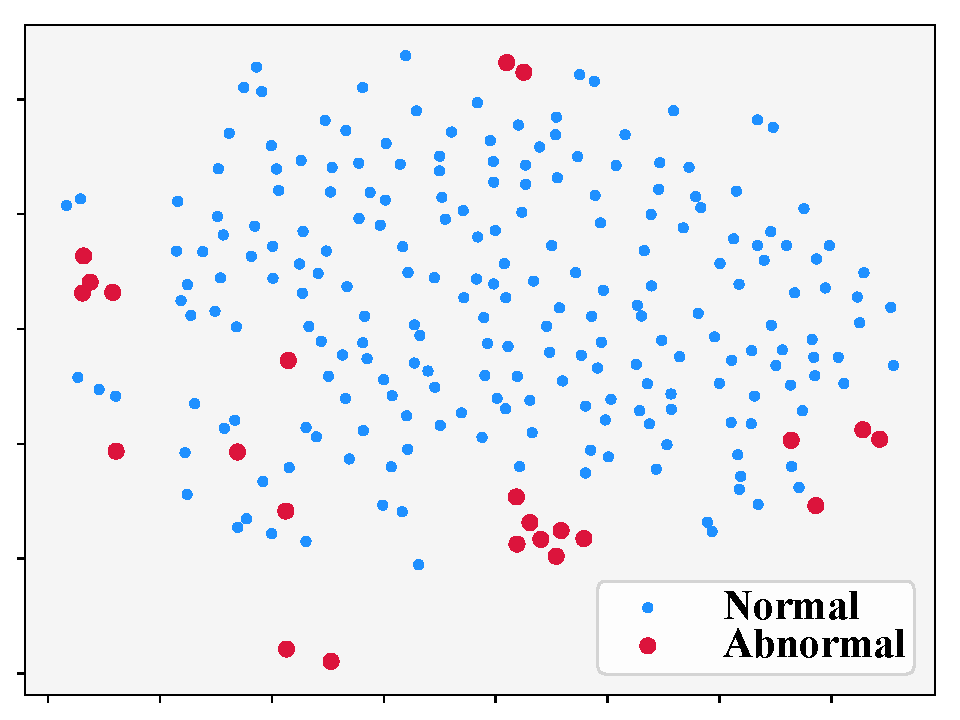
\includegraphics[width=0.3\textwidth]{figures/diverse_tsne}
% 	}
% 	%\hspace{-0.1in}
% 	\subfigure[Similarity Distributions]{\label{subfig:gcn_sim}
% 		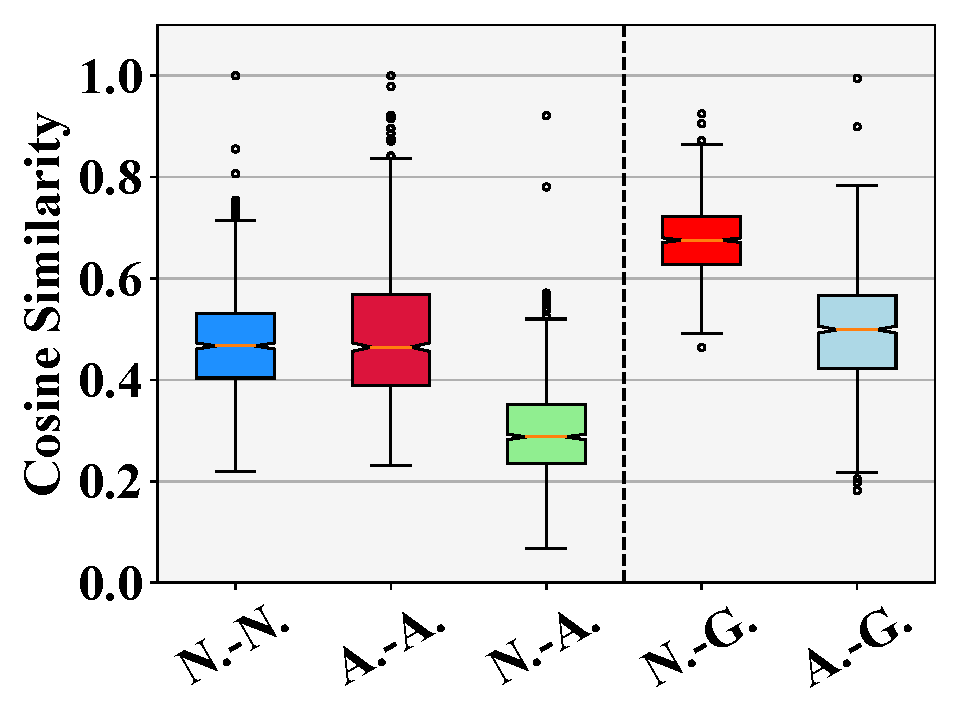
\includegraphics[width=0.3\textwidth]{figures/observe}
% 	}
% 	\caption{\label{fig:para} A real example of detecting the papers (red) that don't belong to ``Jun Lu". %, a professor from University of Munich. 
% 		(a) The t-SNE projection of the graph of all his papers, wherein nodes are papers and if two papers share the same coauthors or venues, an edge links them; 
% 		(b) The similarity between normal nodes and the global context (blue) vs. that between abnormal nodes and the global context (red) by using input features;}  
% \end{figure}





% To further understand the behavior of anomalies, we take the author ``Jun Lu", a professor from Yale University, from Google Scholar's published author profile data as a case study by building a graph with papers assigned to him as nodes, and connect two papers with an edge if they share the same coauthors or venues. 
% The goal here is to detect the wrongly-assigned papers (anomalies), i.e., those that are not authored by him. 
% This anomaly detection problem can be motivated by a news\footnote{https://www.universityworldnews.com/post.php?story=\\20120807160325397} 
% reported in 2012 that another researcher named ``Jun Lu" from Beijing University of Chemical Technology cheated the awards using the papers of ``Jun Lu" from Yale. This event caused by the wrongly-assigned papers of the same author name implies the importance of anomaly detection. Thus, we illustrate how the wrongly-assigned papers can be distinguished from the right ones in Figure~\ref{fig:para}.
% Figure~\ref{sec:intro} (a) shows the t-SNE\footnote{https://lvdmaaten.github.io/tsne/} projection of each node's input features---the BERT embedding~\cite{devlin2019bert} of its title---with blue as normal nodes and red as abnormal ones. 
% We can observe that both abnormal and normal nodes are distributed diversely with abnormal ones being relatively more diverse. As we know, the traditional anomaly detection methods formalize this problem in a classification regime, which aim at learning the expressive node representations and hyperplane to differentiate abnormal and normal nodes. However, based on the case observation, the node distributions, despite abnormal/normal nodes, are too complex for the classier to learn a suitable hyperplane to separate them.   

% However, such anomalies violate the class-homophily assumption in the graph --- two neighboring nodes tend to have similar features and same labels --- via suspicious links, and further hinder the classifiers to learn a efficient hyperplane to differentiate abnormal and normal nodes. 

% the traditional methods formalize the anomaly detection problem in a classification regime, which aim at learning the powerful hyperplane to differentiate abnormal and normal nodes. However, such anomalies violate the class-homophily assumption --- two neighboring nodes tend to have similar features and same labels---and impact the performance of the traditional message-passing along with the links.



% based on the case observation, the node distributions, despite abnormal/normal nodes, are too complex for the classier to learn a suitable hyperplane to separate them.
% Such suspicious links violate the homophily assumption between neighbors---two neighboring nodes tend to have similar features and same labels---and impact the performance of the traditional message-passing along with the links.
% 

 
\begin{figure}[t]
	\centering
	%\hspace{-0.2in}
	%\subfigure[AMiner]{\label{subfig:paper_network}
	%	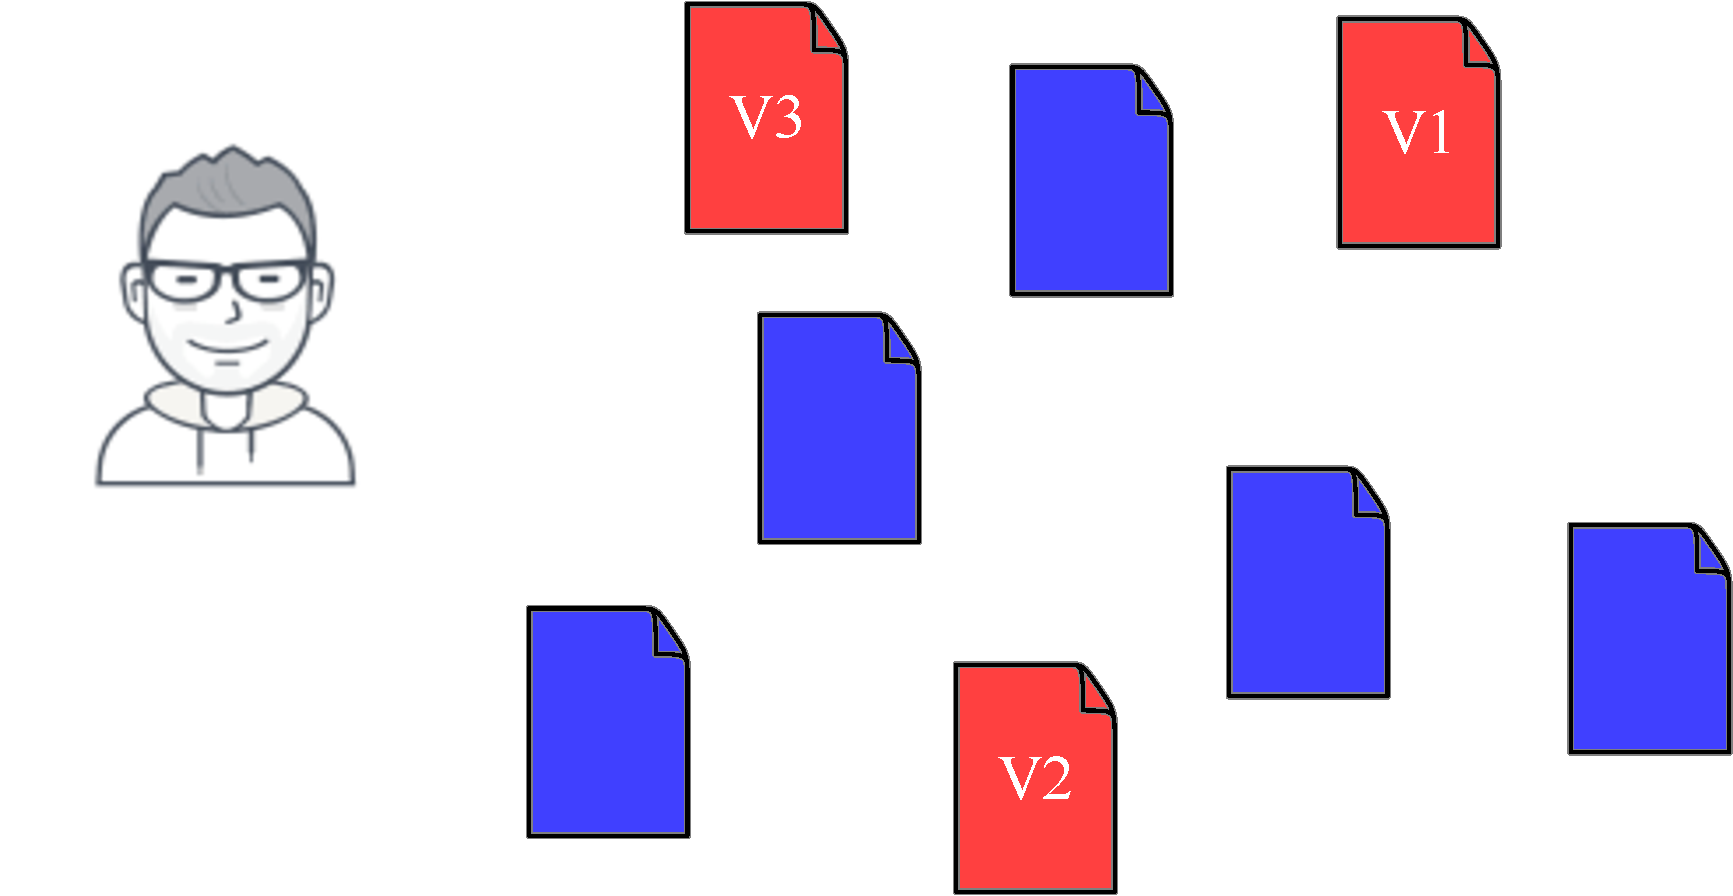
\includegraphics[width=0.33\textwidth]{figures/motivation}
	%}
	\subfigure[t-SNE]{\label{subfig:t-sne}
		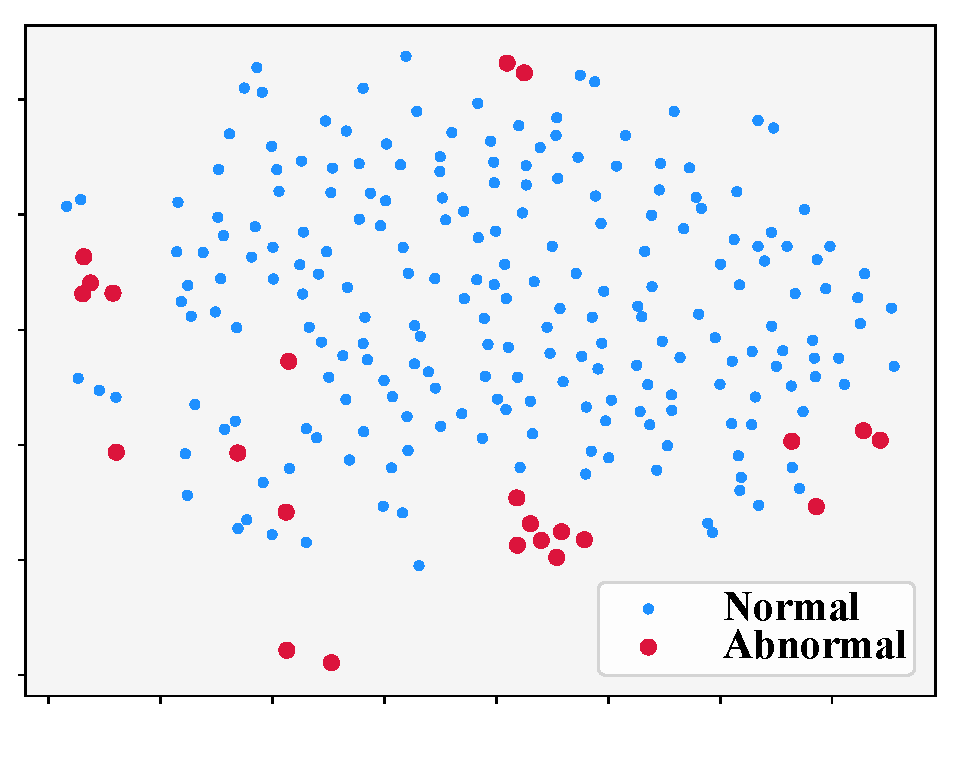
\includegraphics[width=0.205\textwidth]{figures/diverse_tsne_modi.pdf}
	}
	\subfigure[Input Features]{\label{subfig:similarity}
		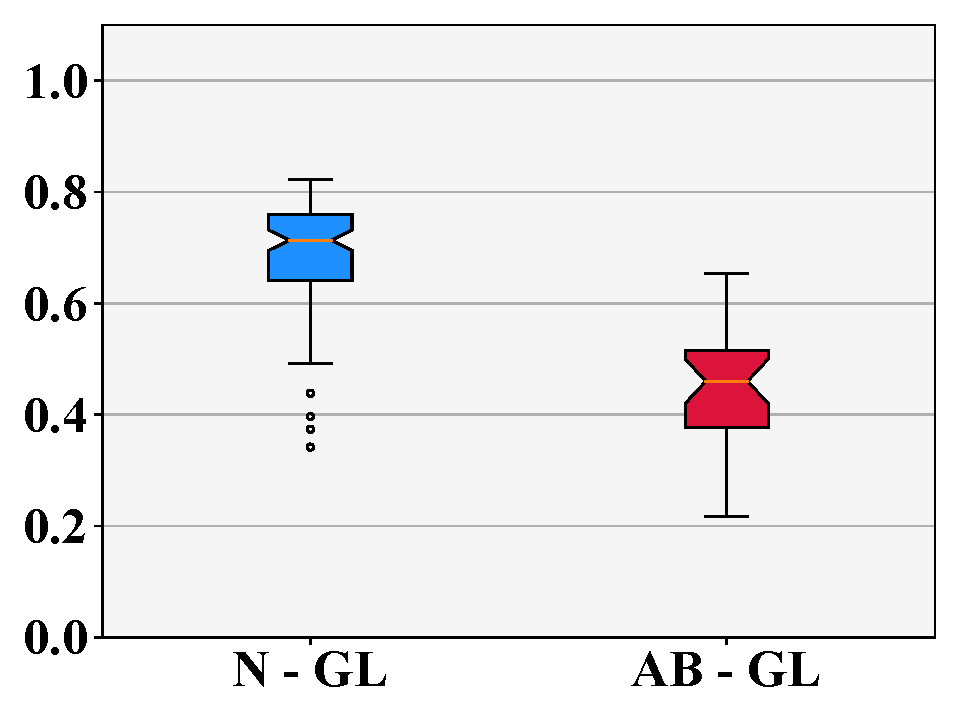
\includegraphics[width=0.21\textwidth,  height=0.121\textheight]{figures/caseBefore.pdf}
	}
	%\hspace{-0.9in}
	\subfigure[Embeddings by GCN]{\label{subfig:gcn_sim}
		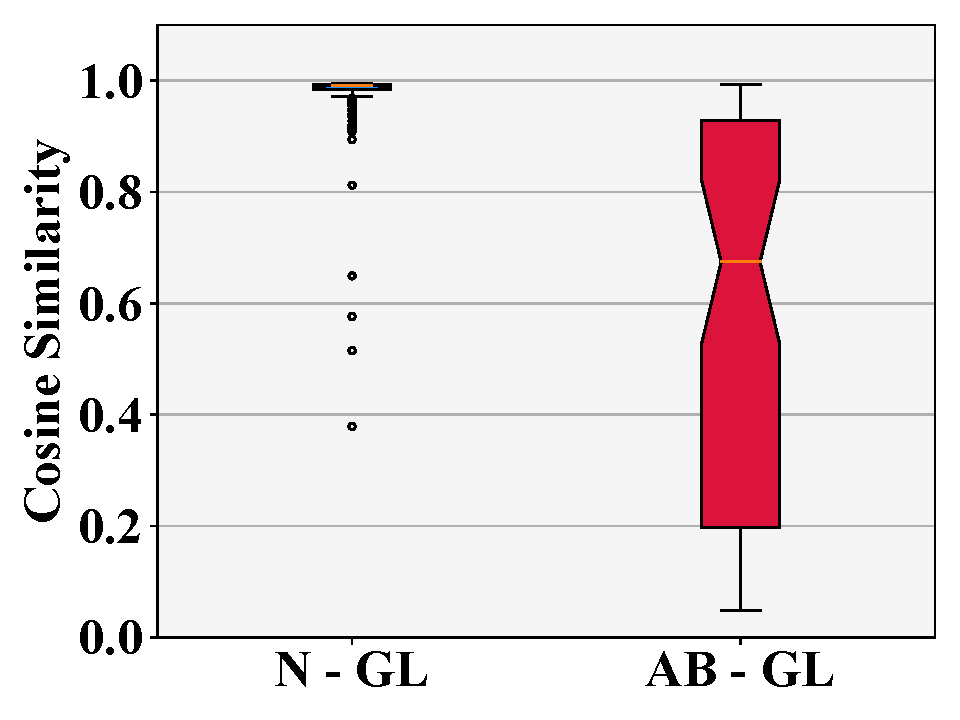
\includegraphics[width=0.22\textwidth]{figures/gcn_diverse}
	}
	\subfigure[Embeddings by \model]{\label{subfig:cogcl_sim}
		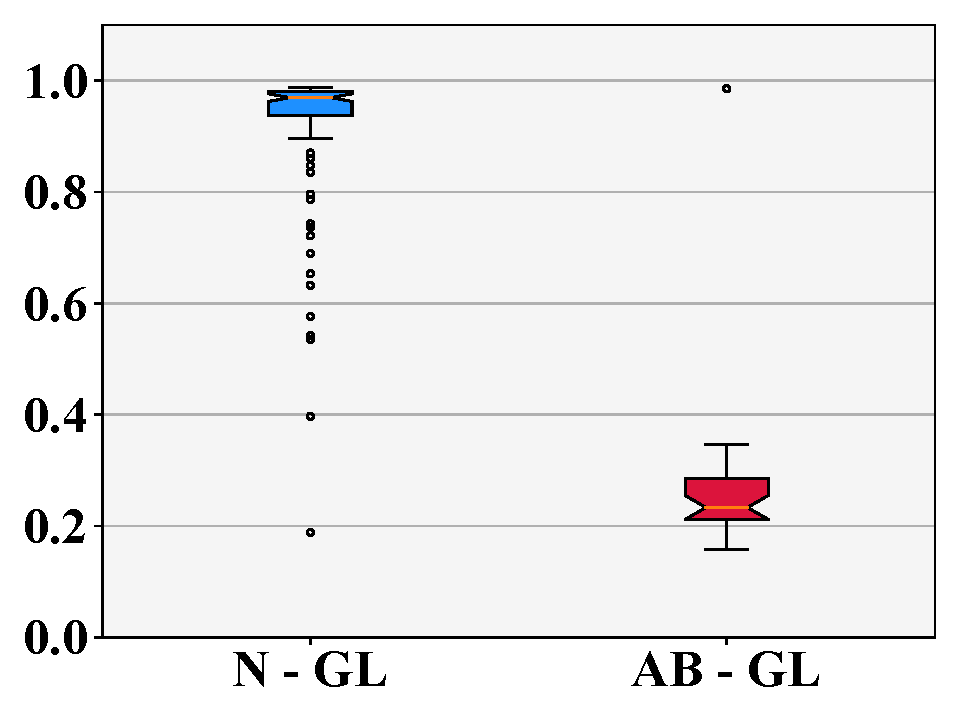
\includegraphics[width=0.21\textwidth,  height=0.121\textheight]{figures/caseAfter.pdf}
	}
	\caption{\label{fig:para} A real example of detecting the papers (red) that don't belong to ``Jun Lu". %, a professor from University of Munich. 
		(a) The t-SNE projection of the graph of all his papers, wherein nodes are papers and if two papers share the same coauthors, affiliations, or venues, an edge links them; 
		(b) The similarities between normal nodes and the global context (blue) vs. that between abnormal nodes and the global context (red) by using input features (N, AB, GL are abbreviated for Normal, ABnormal nodes, and GLobal context, respectively);
		(c) The similarities between embeddings generated by GCN. 
		(d) The similarities between embeddings generated by \model.}  
\end{figure}


To further understand the behavior of anomalies, we take the author ``Jun Lu", a professor from Yale University, from the published author profile of Google Scholar as a case study by building a graph with papers assigned to him as nodes, and connect two papers with edges if they share the same coauthors, affiliations, or venues. 
The goal here is to detect wrongly assigned papers (anomalies), i.e., those are not authored by him. 
This anomaly detection problem can be motivated by a news\footnote{https://www.universityworldnews.com/post.php?story=\\20120807160325397} reported in 2012 that another researcher named ``Jun Lu" from Beijing University of Chemical Technology cheated the awards using the papers of ``Jun Lu" from Yale. This event caused by the wrongly assigned papers of the same author name implies the importance of anomaly detection. Thus, we illustrate how the wrongly assigned papers can be distinguished from the right ones in Fig.~\ref{fig:para}.
Fig.~\ref{subfig:t-sne} shows the t-SNE\footnote{https://lvdmaaten.github.io/tsne/} projection of each node's input features---the BERT embedding~\cite{devlin2019bert} of its title---with blue as normal nodes and red as abnormal ones. 
We observe both abnormal and normal nodes are distributed diversely with abnormal ones being relatively more diverse. 
Intuitively, we quantify this observation by computing the similarity between each node and the global context---the average of all node features%\footnote{The global context is later estimated by the memory-based context updater.}
, which is shown in Fig.~\ref{subfig:similarity}. 
It suggests that though having slight overlaps, the two similarity distributions can be clearly distinguished. 
Inspired by these observations, we explore whether there is a straightforward way to capture them for distinguishing abnormal nodes from normal ones. 




%The study implies that the distance to the global context is  an important but  often neglected factor for detecting the anomalies. 

%Such diverse feature distributions of the normal and abnormal nodes in a graph makes it challenging to find a clear boundary by binary classification, which drives us to explore a more effective solution for anomaly detection.


\vpara{Present Work.} 
In light of the recent progress in contrastive learning~\cite{wu2018unsupervised,he2020momentum}, we propose to contrast each node with the global context of the input graph. 
The underlying assumption is that abnormal nodes tend to be more distant from the majority of nodes, namely the graph context, than normal ones. We name the model as \model, a %\underline{Co}ntext-aware \underline{G}raph \underline{C}ontrastive \underline{L}earning model. 
Graph Contrastive Learning for Anomaly Detection.
Specifically, we design the context-aware graph contrastive loss in a supervised manner, i.e., labeled normal and abnormal nodes are treated as positive and negative keys, respectively (Cf. Section \ref{subsec:overview}), differing it from most existing studies that use graph contrastive learning in a self-supervised pre-training setup~\cite{you2020graph,velickovic2019deep,qiu2020gcc}. 
Fig.~\ref{subfig:cogcl_sim} plots the similarity distributions of embeddings generated by \smodel compared with that by GCN~\cite{kipf2016semi} shown in Fig.~\ref{subfig:gcn_sim}, demonstrating \model's striking capacity of separating abnormal nodes from normal ones when considering their distances to the global context of the graph.


In addition to the supervised \smodel model, we also extend it in an unsupervised pre-training manner \spmodel for handling cases with scarce labels. 
Straightforwardly, we need to synthesize node labels that can be directly used to replace the ground-truth labels in the supervised contrastive loss. 
% To generate synthetic abnormal nodes, 
To achieve this, we design a strategy to corrupt each part of the original graph by injecting the nodes outside this part. 


To achieve the contrastive goal, we propose a context-aware GNN encoder with three modules: \textit{edge update}, \textit{node update}, and \textit{graph update}. 
First, \textit{edge update} is used to estimate the suspicious likelihood of each link and then update the adjacency matrix by removing the most suspicious links. 
Then, \textit{node update} is to update node embeddings by message passing on the updated adjacency matrix. 
Finally, \textit{graph update} is designed to update the global context iteratively. 


We verify the proposed model by two genres of anomaly detection tasks, i.e., detecting wrongly assigned papers in researchers' profiles on two academic datasets --- AMiner and MAS, and detecting users who give fraudulent ratings on two business websites --- Alpha and Yelp. The academic datasets have multiple author profiles where each profile can be viewed as a graph, dubbed as the multi-graph setting. While the business datasets, which have one large graph, are viewed as the single-graph setting.
Experiments show that: 1) \smodel yields substantial improvements on multi-graph datasets, while presenting subtle but consistent performance gain on single-graph datasets compared with state-of-the-art baselines;
2) the unsupervised  \spmodel is comparable with the fully-supervised \model. With further fine-tuning, \spmodel can outperform \smodel on most of the datasets. 
In general, \spmodel yields consistently better performance than other compared graph pre-training methods. The main contributions are summarized as follows:

\begin{itemize}[leftmargin=*]
	
	\item We propose the idea of using graph contrastive learning for anomaly detection and present \smodel by designing context-aware graph contrastive objective. 

	\item We design an effective strategy to yield synthetic labels for extending \smodel to unsupervised \pmodel. 

	%We extend \smodel to \pmodel, a pre-training version in an unsupervised manner, by injecting into a graph the anomalies outside the graph. 
	%Surprisingly, \spmodel can achieve comparable performance with the fully-supervised \smodel without any labeled data in the AMiner dataset.
	\item We devise a context-aware GNN encoder via injecting context information to obtain both node and context representations.
	
	\item We conduct experiments, showing the substantial improvements brought by \smodel and \pmodel. 
	%\item We conduct experiments, demonstrating the significant performance advantages brought by \smodel and \pmodel. 

\end{itemize}




 





















